% THIS IS SIGPROC-SP.TEX - VERSION 3.1
% WORKS WITH V3.2SP OF ACM_PROC_ARTICLE-SP.CLS
% APRIL 2009
%
% It is an example file showing how to use the 'acm_proc_article-sp.cls' V3.2SP
% LaTeX2e document class file for Conference Proceedings submissions.
% ----------------------------------------------------------------------------------------------------------------
% This .tex file (and associated .cls V3.2SP) *DOES NOT* produce:
%       1) The Permission Statement
%       2) The Conference (location) Info information
%       3) The Copyright Line with ACM data
%       4) Page numbering
% ---------------------------------------------------------------------------------------------------------------
% It is an example which *does* use the .bib file (from which the .bbl file
% is produced).
% REMEMBER HOWEVER: After having produced the .bbl file,
% and prior to final submission,
% you need to 'insert'  your .bbl file into your source .tex file so as to provide
% ONE 'self-contained' source file.
%
% Questions regarding SIGS should be sent to
% Adrienne Griscti ---> griscti@acm.org
%
% Questions/suggestions regarding the guidelines, .tex and .cls files, etc. to
% Gerald Murray ---> murray@hq.acm.org
%
% For tracking purposes - this is V3.1SP - APRIL 2009


\documentclass{sig-alternate}

\usepackage[lined,ruled,commentsnumbered,linesnumbered]{algorithm2e}
\usepackage{epstopdf}
\pagenumbering{arabic}
\newtheorem{theorem}{Assumption}

\begin{document}

\title{Adaptive Model-Based Policy Translation for Usage Control}
%
% You need the command \numberofauthors to handle the 'placement
% and alignment' of the authors beneath the title.
%
% For aesthetic reasons, we recommend 'three authors at a time'
% i.e. three 'name/affiliation blocks' be placed beneath the title.
%
% NOTE: You are NOT restricted in how many 'rows' of
% "name/affiliations" may appear. We just ask that you restrict
% the number of 'columns' to three.
%
% Because of the available 'opening page real-estate'
% we ask you to refrain from putting more than six authors
% (two rows with three columns) beneath the article title.
% More than six makes the first-page appear very cluttered indeed.
%
% Use the \alignauthor commands to handle the names
% and affiliations for an 'aesthetic maximum' of six authors.
% Add names, affiliations, addresses for
% the seventh etc. author(s) as the argument for the
% \additionalauthors command.
% These 'additional authors' will be output/set for you
% without further effort on your part as the last section in
% the body of your article BEFORE References or any Appendices.

\numberofauthors{2} %  in this sample file, there are a *total*
% of EIGHT authors. SIX appear on the 'first-page' (for formatting
% reasons) and the remaining two appear in the \additionalauthors section.
%
\author{
% You can go ahead and credit any number of authors here,
% e.g. one 'row of three' or two rows (consisting of one row of three
% and a second row of one, two or three).
%
% The command \alignauthor (no curly braces needed) should
% precede each author name, affiliation/snail-mail address and
% e-mail address. Additionally, tag each line of
% affiliation/address with \affaddr, and tag the
% e-mail address with \email.
%
% 1st. author
\alignauthor
Ciprian Lucaci\\
       \email{lucaci@in.tum.de}\\
 	 \affaddr{Technische Universit{\"a}t M{\"u}nchen, Germany}
% 2nd. author
\alignauthor
Prachi Kumari\\
       \email{prachi.kumari@in.tum.de}\\
 	 \affaddr{Technische Universit{\"a}t M{\"u}nchen, Germany}
}
% There's nothing stopping you putting the seventh, eighth, etc.
% author on the opening page (as the 'third row') but we ask,
% for aesthetic reasons that you place these 'additional authors'
% in the \additional authors block, viz.

% Just remember to make sure that the TOTAL number of authors
% is the number that will appear on the first page PLUS the
% number that will appear in the \additionalauthors section.

\maketitle
\begin{abstract}
Adaptive Model-Based Policy Translation for Usage Control abstract
This paper provides a sample of a \LaTeX\ document which conforms to
the formatting guidelines for ACM SIG Proceedings.
\end{abstract}

% A category with the (minimum) three required fields

%A category including the fourth, optional field follows...

\keywords{Usage Control, Adaptive Systems} % NOT required for Proceedings

%===========================================
% INTRODUCTION
\section{Introduction}
Usage control is a generalization of access control that specifies and enforces what 
must or must not happen to data once access to it has been granted. 
Some example policies include ``delete data after 30 days'', ``don't distribute my data'', ``don't copy data without permission''.
Policies are supposed to be specified by end-users and translated using technical details provided by a more sophisticated user, whom we call the power-user \cite{proceeding4}. 
A policy consists of a set of data (e.g. picture, email, document), 
a set of actions (e.g. print, copy, distribute, save) and constraints (e.g. maximum times, do not, after some time).
These policies, specified by an end user in terms of abstract data and actions, are called the specification-level policies (SLP) \cite{proceeding5}. 
Specification-level policies describe what must and must not happen throughout the execution of a system. 
For enforcement, SLPs are translated into implementation-level policies (ILP) with concrete representations of the abstract data and actions achieved through model based refinement. 
Implementation-level policies refine them by stating how they will actually be enforced.
ILPs are enforced at, and across each layer of abstraction in each machine in a distributed system. 

In the existing work on policy translation, the refinements of data and action are defined at the level of the domain. 
The domain meta-model \cite{proceeding5}, shown in Figure~\ref{fig:metamodel}, consists of three layers:
the platform-independent layer (PIM), that is to be defined and used by the end-user;
the platform-specific layer (PSM), that is to be defined and used by the so called power-user;
and the implementation-specific layer, also to be defined and used by the power-user, that reflects the technicalities of the system on which the policies are to be deployed.
Our domain meta-model, distinguishes among user-intelligible high-level actions on data like ``copy photo'' at the platform-independent (PIM) layer,
refined as implementation independent technical representations (called transformers) like ``take screenshot'' at the platform-specific (PSM) layer,
and the specific implementations of these transformers like ``getImage()'' function in the X11 windowing system at the implementation-specific (ISM) layer \cite{proceeding4}.

The previous work had one basic assumption behind, namely the domain structure is static. 
This means that we have assumed that all components in the domain and their relationships with one another
 at various levels of abstraction are known and specified beforehand. 
However, in real world, domains evolve over time with services, logical systems and physical hosts being added, removed or modified.
Let us consider an online social network (OSN) example:
new components can be introduced and various existing components can be modified with new features of social networking, 
e.g. the ad-service can be provided by the OSN provider or can be outsourced;
various third-party applications can hook into the OSN, a new browser could be installed, and so on.
The client machines accessing the social network at various users' end might also change in their technical configurations. 

\begin{figure}
\centering
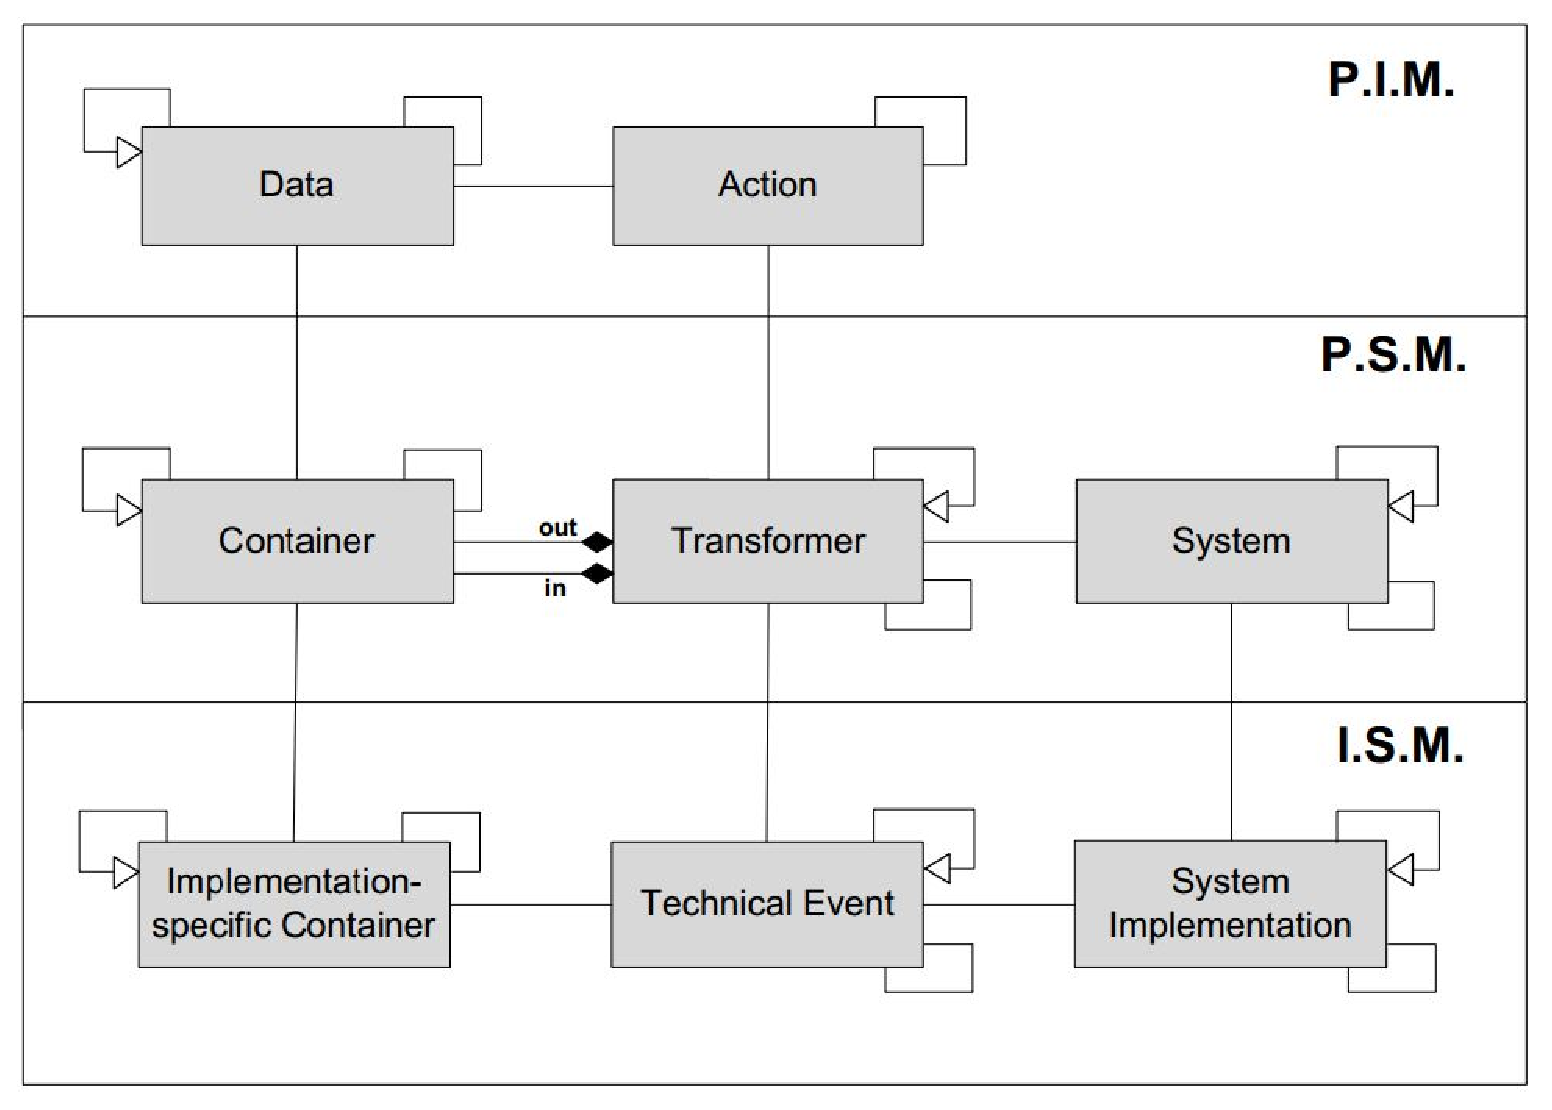
\epsfig{file=domain-meta-model.eps, height=2in, width=3in}
\caption{Domain meta-model}
\label{fig:metamodel}
\end{figure}

\textbf{Research problem} 
Any realistic policy translation, therefore, must reflect these changes. 
So the first question that must be answered is: (1) how can we recognize changes in the domain structure? 
It is obvious that any changes in the domain structure must be reflected in the domain model that is used for data and action refinements. 
So the second requirement is about decision making: (2) how do we decide if the changes are to be accommodated in the policy translation
and at what levels in the domain model must these changes be included? 
The third part of the problem is about (3) applying the changes. Intuitively, adding and removing refinements from the domain model is trivial. 
Updating the refinements however might not be straightforward.
This subproblem therefore will be addressed by coming up with ways of merging different refinements of the same data or action and reflect the new refinements in the translation. 
This means that new policies must be generated or the already deployed policies need to be revoked and the new changed ones must be deployed.

\textbf{Solution} 
In the following paragraphs we present the solution to the problems presented before. 
For successfully overcoming the problems we employ techniques found in adaptive systems and also concepts from ontology merging. 

%===========================================
% CONCEPTUAL
\section{Conceptual}

To better understand the requirements of an adaptive system we used the approach described in \cite{proceeding10},
and thus we identified the goals, the uncertainty factors and how to mitigate them. 
The top-level goal, which states the overall objective is represented by the achievement of the update of the domain model (DM); 
the lower-level goals, which contribute to the high-level functionality, are to identify when the DM has changed and what cases of changes there are; 
the uncertainty factors are represented by the potentially conflicting requirements, i.e. two conflicting refinements; 
and the mitigation of the uncertainty factors is represented by the adaptation behaviour.

In the following paragraphs, we use the term \textit{Base Domain Model} (BDM) for the domain-model which has to be updated
and the term \textit{New Domain Model} (NDM) for the model which contains the updates.
After update, the BDM contains the domain model used for policy translation.
The same name pattern is applied also in the context of data, containers, actions, transformers and systems.

%----------------------------
\subsection{Ontology merging}
An ontology typically provides a vocabulary describing a domain of interest and a specification of the meaning of terms in that vocabulary.
As presented in \cite{book1} the matching operation is the process of finding relationships or correspondences between entities of different ontologies.
The matching of two ontologies can be done by using different techniques applied at different levels, such as element-level or structure-level.
From the matching techniques described in \cite{book1} we use both element-level and structure-level approaches.
Also the matching process takes into consideration linguistic properties, internal properties and semantic properties.
These properties are described in detail for each type of elements in the domain model in the following sections.
The ontology merging process is the creation of a new ontology from two, possibly overlapping, source ontologies. 
The merged ontology is assumed to contain the knowledge of the initial ontologies, e.g., consequences of each ontology are consequences of the merge. 
This concept is closely related to that of schema integration in databases \cite{book1}. 
In our case, the ontology is represented by the Base Domain Model and the New Domain Model consisting of PIM, PSM, ISM elements,
which have to be matched and merged.

\cite{proceeding11} studies possible relationships between concepts in adaptive web systems.
By applying these relationships between the elements in the domain model, one can easily see that there are essentially only two types of relationships
that we have to consider for merging both data/containers and action/transformers: \textit{containment} and \textit{equivalence}. 

\textbf{\textit{Containment(a,b):}} \textit{Concept a contains concept b if and only if b is held within concept b.}

\textbf{\textit{Equivalence(a,b):}} \textit{Concept a is equivalent to concept b if and only if they are essentially equal.}

These relationships are further defined in the context of data/containers, action/transformers and systems.
They take into considerations the following information: 
\textit{syntactic information}, given by the name and the type of the element, e.g. a data can be merged only with a data, an action only with an action;
\textit{structural information}, given by the type of refinement, e.g. sequence refinement can be merged only with another sequence, and set with set; 
and \textit{semantic information}, provided by the refinement elements or the synonymity of terms. 
 
While merging, the first assumption, Assumption~\ref{assumption1}, that we consider implicit is that merging is done only at the same layer of abstraction, i.e. PIM-PIM, PSM-PSM, ISM-ISM. 
It also means that only elements pertaining to the same system are merged. 
For example, when merging a file system details with another file system details at the PSM level, we never merge these details with those of a database system;
similarly, when merging Firefox with Firefox details and Unix system calls with Unix system calls at the ISM level. 

%----------------------------
\subsection{Adaptive systems}
Self-adaptive systems have in common that they can reason about their state and environment. 
This is done via feedback processes described by a control loop which describes four key activities: collect, analyse, decide and act \cite{adaptive1}.
These four key activities are captured by the three questions introduced in the beginning.
Collect is represented by \textit{Recognize}, 
analyse and decide is represented by \textit{Decide},
and act is represented by \textit{Incorporate}.
Therefore, for each layer of abstraction the changes have to be recognized, the information must be analysed and the merging must be applied, and all in an automatic manner.

In order to accommodate changes at each layer of abstraction, each layer must be seen as an adaptive system which must react to change.
Therefore, to reach the top-level goal, a fully decentralized pattern seems to best fit the use case, as seen in \cite{adaptive2}. 
This means that from a conceptual perspective, there is a control loop at each level (PIM, PSM and ISM)
and when an event to adapt comes, the levels inform each other of the required change.

Having considered all these, a generic algorithm which achieves the top-level goal of merging two domain models is Algorithm~\ref{algo_generic}.

\IncMargin{1em}
\begin{algorithm}
  \SetKwInOut{Input}{input}\SetKwInOut{Output}{output}
  \Input{baseLayer, newLayer :domain model layer}
  \Output{baseLayer :domain model layer}
  \BlankLine
  	\emph{/* Stage 1. Recognize new elements */}\;
  	\ForAll{elements of $newLayer$}{
  		\emph{/* makes use of the equivalence(a,b) relation */}
  		baseE = searchEquivalent(newE, baseLayer)\;
  		\If{equivalentExists == false}{
		      add newE to baseLayer\;}
                updateInnerLayerRefinement(baseE, newE)\;
    	}  	   	
  	\emph{/* Stage 2. Decide */}\;
  	\ForAll{elements of $newLayer$}{
  		baseE = searchEquivalent(newE, baseLayer)\;
                updateCrossLayerRefinement(baseE, newE)\;
    	}    		
	\emph{/* Stage 3. Incorporate */}\;  
	\ForAll{elements of $baseLayer$}{
	  	\emph{/* makes use of the containment(a,b) relation */}
  		removeRedundantRefinement(baseE);
    	}   
  \caption{Generic merge}\label{algo_generic}
\end{algorithm}
\DecMargin{1em}

Further we will present every step (i.e. recognize, decide, incorporate) necessary to obtain the merging applied at the level of data and containers, actions and transformers and systems.


%===========================================
% SUBSECTION
% DATA/Containers
%----------------------------
\subsection{Data and Containers}
The first uncertainty factor is represented by the possible changes in the domain model.
Therefore the first step towards mitigation is to identify all the possible changes from PIM level to the ISM level.
The domain model can change by addition of elements, removal of elements or modification of the relations between the elements, i.e. associations.
In the context of data and containers, adding new elements means for the end-user the addition of new elements which can later be used as elements for the policy specification; 
e.g. add ``profile'' data at PIM, ``file'' container at PSM or ``unixFile'' at ISM.
Modifying the relations means changing the semantics of the domain-model,
e.g. before, a ``profile'' was composed only of a picture, and after adaptation, a ``profile'' is an aggregation of ``pictures'' and ``comments''.
These types of changes can appear at each level of the domain, and we will expand upon them.
At the same time one must also investigate how the changes are affecting each other, if or how they affect multiple levels of abstraction.

%----------------------------
\subsubsection{Recognize Changes}

At the level of Platform Independent Model (PIM) the first type of change is represented by the addition of a \textit{new data}.
This can come in different versions. 

First, if the New Data (ND) is refined in terms of other existing Base Data (BD) at the PIM level then the adaptation affects only the PIM level, no further updates are necessary.
This is a case when only an association between data changes
when the associations between data and data, named \textit{inner-layer associations}, might need to be updated,
as it was in the aforementioned example of adding a ``comments'' element to a ``profile''.
The associations between data can be of type \textit{aggregation}, an album is an aggregation of pictures, and \textit{composition}, a table is a composition of rows.
Also, some of the associations between ND and Base Action (BA) at PIM have to be updated, meaning that there might be actions which can apply on the new data.
If the new domain model (NDM) consists only of modified associations or removal of elements, the same pattern of actions can be applied.
Besides these updates, no other levels are affected.

Secondly, when a New Data needs to be added to the Base Domain Model (BDM),
besides the updates presented before, also associations between the New Data (ND) at PIM and the Base Container (BC) at Platform Specific Model (PSM) might need to be updated.
This is a case of \textit{cross-layer associations} between data and container.
An example of this could be an addition of ``picture'' at PIM which is refined as a ``file'' at PSM.
Additionally, if the PSM container does not exist, then a new container at PSM level needs to be added first.
Then, the necessary associations at PSM level between existing transformers and the new container need to be updated in a similar manner with those at PIM.
Only as the last step the cross associations between PIM data and PSM container can and must be added.
This is an example where a change at one layer affects also another layer.

Thirdly, it might be the case that the New Container at PSM from the previous step is part of a new system, e.g. distributed file system.
In this case, the actual implementation of this container needs to be specified also at the ISM layer because PSM layer contains no implementation details.
Therefore, if the ISM containers do not exist, the necessary containers at ISM level have to be added,
together with the inner and cross layer associations. 
This is a example when a change at PIM requires a change at PSM, which in its turn, requires a change at ISM.
All the three layers are affected. 
An example of this could be the addition of ``video'' data at PIM, 
which requires a new container such as ``htmlElement'' at PSM,
which in its turn is refined as ``video'' label in html5.

At the PSM and ISM level the same patters of changes and effects are applied for the addition of containers
and the update of the inner/cross layer associations between containers and transformers
or the associations between containers and transformers.
All the events involved with adding, changing or removing a data or a container are essentially the same for all the layers.

One can immediately observe that the flow of changes is from top to bottom.
A change in a lower layer does not imply a change in the upper layer.
This is because the level of abstraction decreases from top to bottom,
meaning that PIM is an abstraction of PSM, and PSM is an abstraction of ISM, 
or in other words, PSM provides technical details for the PIM layer and ISM provides implementation details for PSM.
The relation across layers data-container and container-container is of type generalization-specialization,
the relation inside the same layer, inner-layer association, is of type aggregation or composition.
The inner-layer associations between data reflect the associations between real systems,
such as a database or an excel document where a workbook is composed of tables,
a table is composed of rows, a row is composed of cells; 
or in a file system where a directory can be an aggregation of files;
or a html page which is an aggregation of html elements which in their turn are refined as labels, tables, forms and these can contain other html elements.
The cross-layer associations  between concepts reflect how the data is stored in real systems, 
or how technical concepts are implemented in particular systems. 
In this context, we mention that refinement of an element means providing technical details or implementation details from a lower level of abstraction.

\begin{figure}
\centering
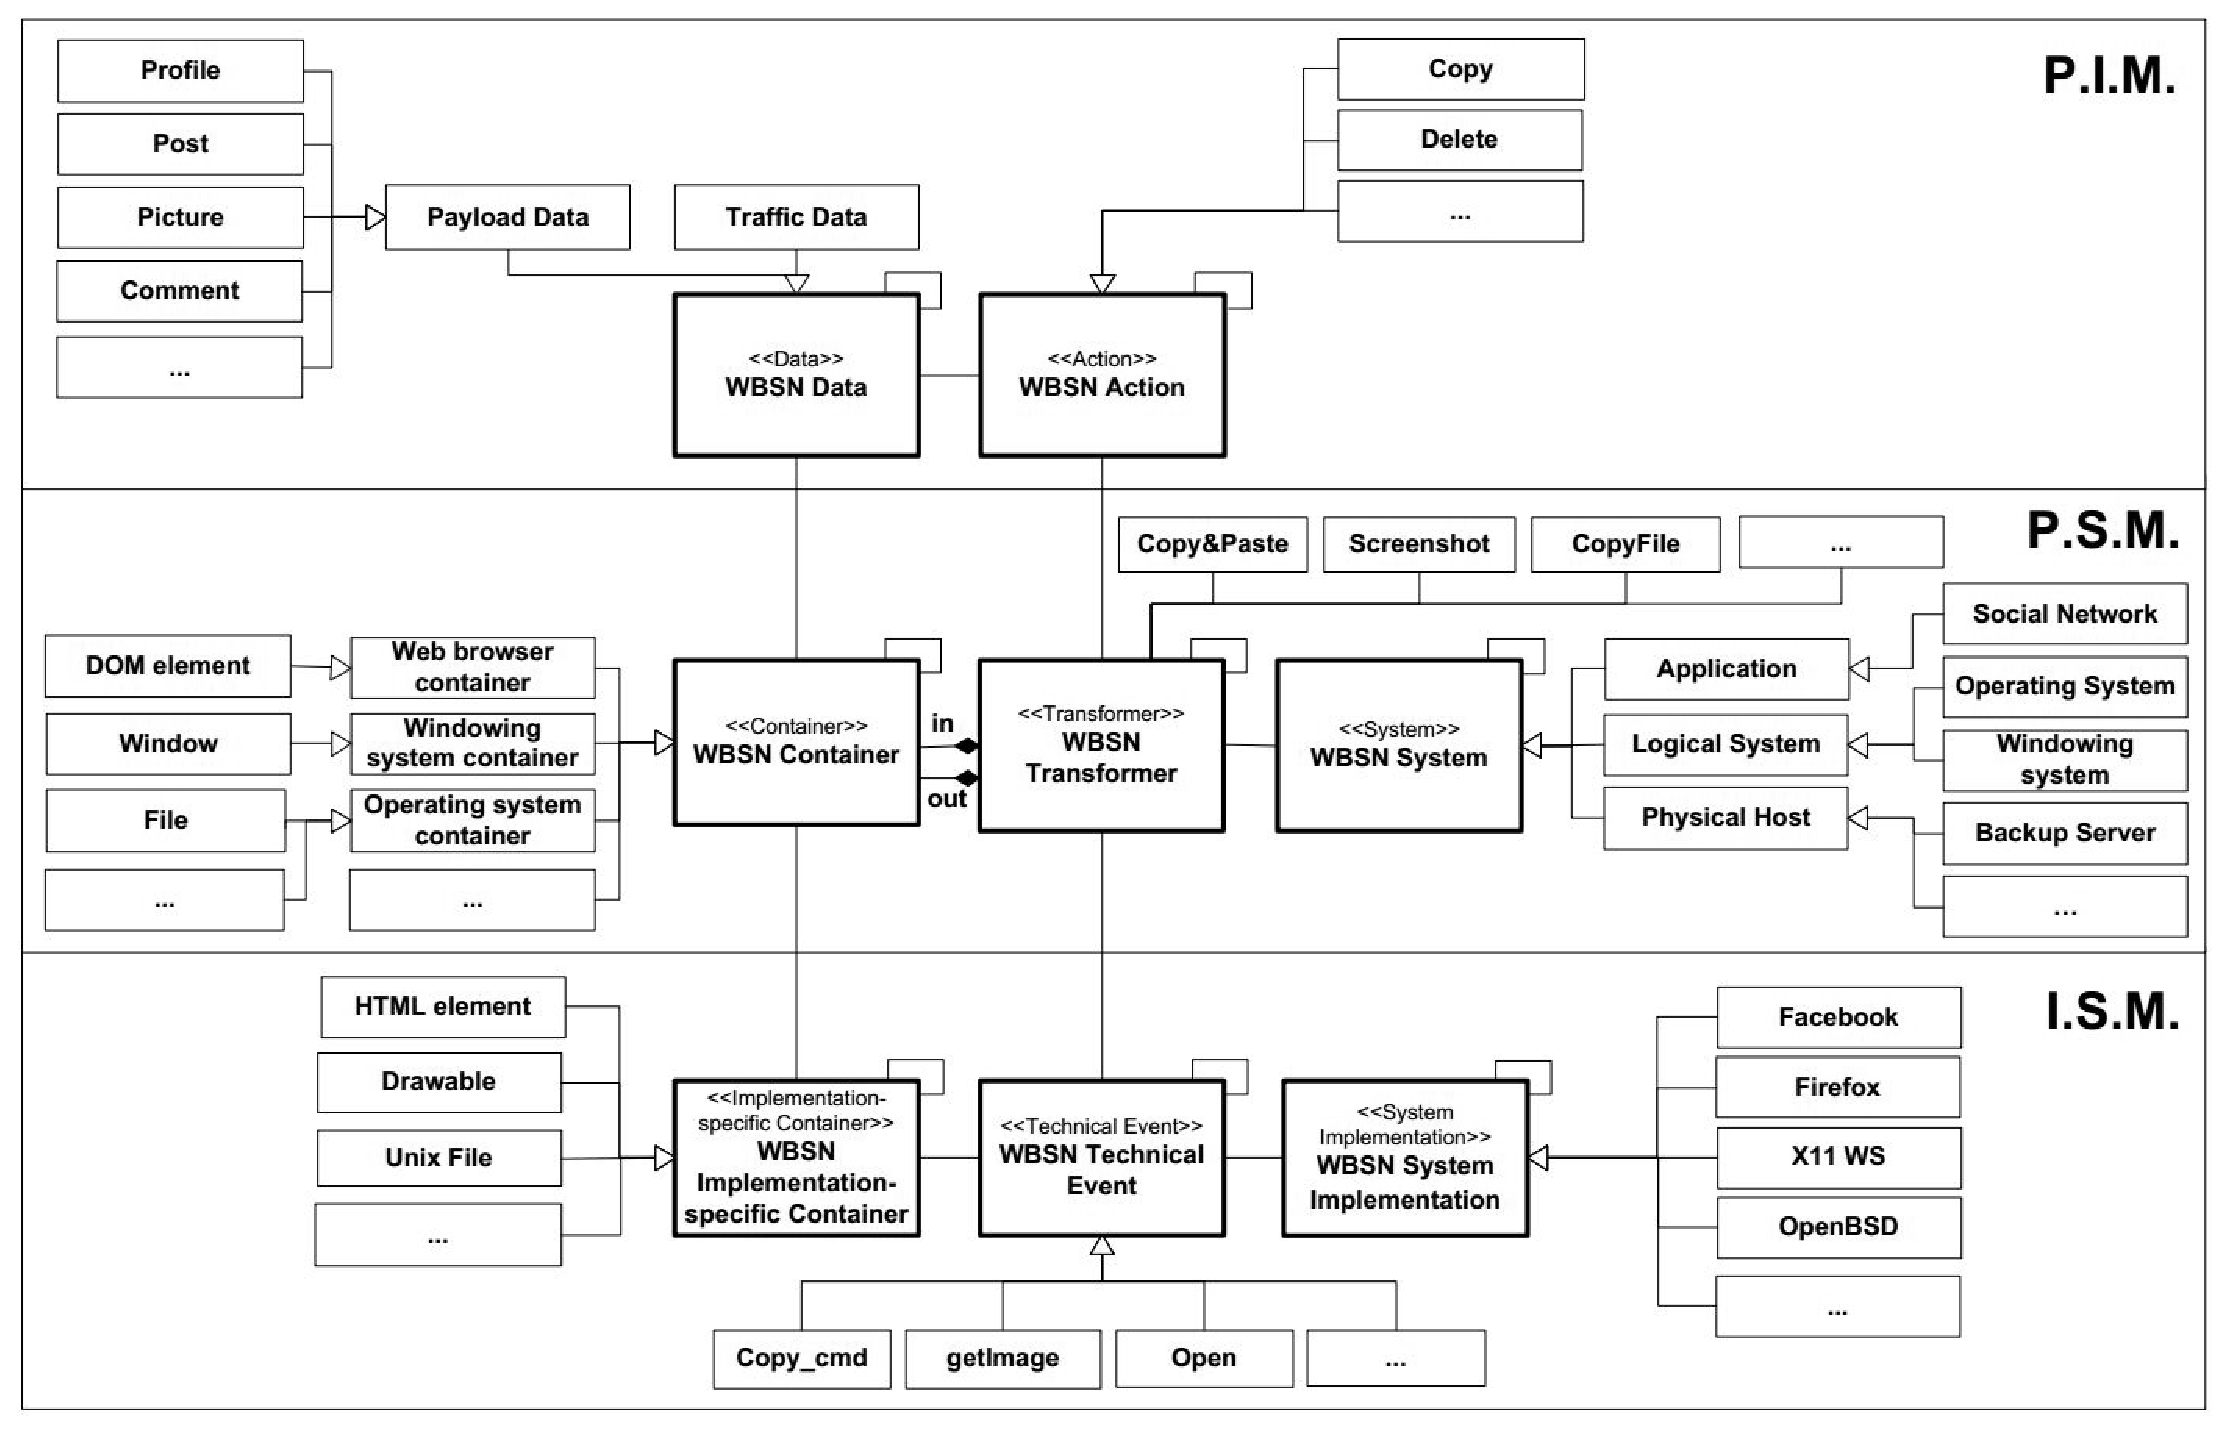
\epsfig{file=wbsn_dm.eps, height=2in, width=3in}
\caption{Online Social Network - domain model}
\label{fig:metamodel-instance}
\end{figure}

\subsubsection{Decide upon Changes}

We have seen that in order to achieve ontology merging, one has to establish relationships between elements.
These relationships can be of type \textit{containment} and \textit{equivalence}.
To establish a relationship between two elements, one can use syntactic, structural or semantic information.

In the case of data, the \textit{syntactic information} is given by the term used to label an element.
Therefore, if two data, one from the base domain and the other from the new domain,
have the same name, then these two containers represent the same container.
Therefore, in the case of data the syntactic information is given only by the name for the following reasons.
Data is specific to a particular user's domain model. The PSM layer containers represent only where can that data be stored.
The same data from different domain models can be stored in different containers and in different implementations.
This does not necessarily mean that the data is different, but only that it can be stored in different containers.
Also, the same label can be used by different users in two different domain models to store different information in the same container.
Having no other information available in the domain model, one has to assume that the same term is used with the same meaning
in different domain models if these domain models are to be merged.
With regard to \textit{structural information}, data and containers are refined only as a set of other elements.
For the reasons mentioned before, no information can be used to establish the relationship between the elements only by using the refinement.
Considering the \textit{semantic information} in the case of data, this is given by lexical similarity between the names of the two data.
For example, in the base domain a data is labelled ``picture'', whereas in the new domain, the same data is labelled ``photo'', 
the two labels are in a relationship of synonymity from a lexical viewpoint.

In the case of containers, the \textit{syntactic information} and the \textit{structural information} is the same as in the case of data.
The difference comes at the \textit{semantic information} where for PSM and ISM containers no lexical information can be established for the following reasons.
When considering the PSM and ISM levels one has to keep in mind that these represent generic systems at PSM level and actual system implementations at ISM level. 
Additionally, to ensure a basic level of compatibility between domains one has to consider at PSM and ISM the terminology for containers and transformers
to have a rather fixed or stable terminology for the same systems.
For example, a container named ``file'' remains ``file'' for all generic operating systems (OS).
There should not be two ontologies which talk in different terms about an OS system, 
i.e. in one case there is ``file1'' and in the other one there is ``file2'' for the same container.
Of course, there are differences at ISM level for  different implementations of the OS, such as Windows or Unix.
Therefore at PSM, for the same system, one has to use the same terminology for all domain models.
At ISM level, if the names differ, this means they represent two different implementations, e.g. open and fopen, exec and execv.
We consider this to be a reasonable assumption, see Assumption~\ref{assumption3}.

Further, we acknowledged that there is no \textit{containment} relation between data-data or container-container when considering merging.
Although, in the same domain model there can be aggregations and compositions defined, thus containment relationships,
these relationships are defined at the structural level and not at the lexical level.
These types of relationships will be automatically merged when considering the refinement or the associations defined in the domain model.
For example, an ``album'' at the lexical level is related with a ``picture'', an album contains pictures, 
but this has to be defined in the domain model and not inferred from the terms.

In terms of refinement, the result refinement is the superset of the lower level containers
because the refinement has no influence upon the relationships between data and/or containers.
If ``picture'' was refined only as an htmlElement at PSM and the new model refines ``photo'' as file,
the result will be ``picture'' refined as htmlElement and file. 
The new domain model is always an update of the base one, not a replacement.

Therefore, two data are \textit{equivalent} if the names are the same or synonymity can be established between them.
Two containers are equivalent only if the names are the same.
The merging is done based on the name of the data or the name of the container.

\textbf{\textit{Equivalence(a,b):}} \textit{Data or container a is equivalent to data or container b if and only if they have the same name or the names are synonyms.}

%----------------------------
\subsubsection{Incorporate Changes}

We have already seen that the flow of changes is from top to bottom.
More specifically, if one wants to add a data, first the refinement elements of the lower levels must be added first.
Therefore, when incorporating the changes, one has to use a bottom-up approach,
add the lower elements first and only after that merge the upper elements based on name and merge the refinement.
By using the patterns and activities described in \cite{adaptive1, adaptive2} the adaptation process applies the following steps at each layer, see Algorithm~\ref{algo_dc_merge} 

\IncMargin{1em}
\begin{algorithm}
  \SetKwInOut{Input}{input}\SetKwInOut{Output}{output}
  \Input{baseLayer, newLayer :domain model layer}
  \Output{baseLayer :domain model layer}
  \BlankLine
  	\emph{/* Stage 1. Recognize */}\;
  	\ForAll{elements of $newLayer.DataCont$}{
  		\emph{/* makes use of the equivalence(a,b) relation */}
  		baseE = searchEquivalent(newE, baseLayer)\;
  		\If{equivalentExists == false}{
		      add newE to baseLayer\;}
                updateInnerLayerRefinement(baseE, newE)\;
    	}  	   	
  	\emph{/* Stage 2. Decide */}\;
  	\ForAll{elements of $newLayer.DataCont$}{
  		baseE = searchEquivalent(newE, baseLayer)\;
                updateCrossLayerRefinement(baseE, newE)\;
    	}    			
  \caption{Data and Containers merge}\label{algo_dc}
\end{algorithm}
\DecMargin{1em}

We start by illustrating at ISM.
In \textit{Stage 1}, all the new ISM containers from the new domain model are added to the base domain model.
For each new container, its counterpart is searched in the base domain. 
But before doing any merging, for each new container the same procedure is applied for every refinement.
In this manner we ensure that the most concrete containers are added first, and then the algorithm returns in a recursive manner to merge the containers.
If the container is already a leaf in the tree of refinements, than no recursive call on its refinements can be made. 
At this step, the new container is compared with each base container by comparing its name.
As we have already mentioned, see assumption~\ref{assumption3}, at ISM level containers are matched by the same name.
If the base container does not exist, than the new container is added to the base.
Next, the inner-layer associations are added.
For example, before adaptation the base domain had the container ``file'' and the container ``htmlElement'' which was associated with ``img'' container only.
The new domain container ``htmlElement'' is associated with ``label'' and ``media'', while ``media'' is associated with ``img'' and ``video''.
After this step is finished the base domain model will be the following: ``file'', ``htmlElement'' associated with ``label'' and ``media'', and ``media'' associated with ``img'' and ``video''. 
One can observe that the old containers were kept and the new associations have been updated.
The same strategy is applied also at PSM with no difference because the assumption~\ref{assumption3} is valid there also.

In \textit{Stage 2} we process the cross layer associations.
After the previous step, all containers from the new domain model are now present in the base domain model.
Also, all the inner associations between containers are present.
The next step is that for each container, at PSM to add the cross layer associations.
For each new container from the new domain and for each cross layer association of that container,
the association is added to the corresponding base domain container. 
There is no need to check if the container is present, because this was already done in the first stage.
Now that the ISM and PSM layer are completely merged, we can proceed to the final stage.

In \textit{Stage 3} the PIM data of the base domain model and new domain model are compared.
We apply the same steps starting from stage 1 with a few differences. We will expand only on the differences.
The inner-layer associations at this level can be of two types, aggregations and compositions, but this does not affect the merging.
Next, for all data containers from the new domain model is searched a counterpart in the base domain model. 
The first step of the search is to look for a container with the same name or a synonym.
If there is no match, than a lexical library is used to compute a similarity metric between the words that form the name of the compared containers.
The closest base concept to the new concept is chosen as the container for the merging.
If two concepts, names are similar, than the base container will from now on also contain a synonym name;
we introduce here the concept of an ``alias'' to the the name of an element, an alias is a synonym in this context.
This is done in order to optimize the adaptation process for a future adaptation event, 
but also if a policy is specified in the terms of the new data, now the translation engine can translate automatically based on the alias.
The final step is to add the cross layer refinements as described in stage 2.

One can immediately observe that there are no merging exceptions. 
This is because the semantic of containers is based only on the names of the containers.
At the ISM and PSM level there is a common terminology, and each new term is considered a new feature of the system.

A final remark in this section is that if a container is added, this most likely implies a change also on the transformers side.
It is highly unlikely to add only a container and no transformers.
Transformers, by definition are applied on a set of containers and the represent system functions.
For example, transformers that work on a container ``file'', will not work on another type of container.
Transformers at PSM and ISM level are closely related with real systems. 
System functions have limited set of data types on which they can be applied.
Usually, a new container is related with a new system, thus, new transformers have to be added also.
On the other hand, if one adds a new transformer, no new containers are usually required.
In general, new transformers add new functionality on the existing containers.
With this in mind, we continue to the next adaptation context, systems.

%===========================================
% SUBSECTION
% Systems
\subsection{Systems}
Systems are present at the PSM level, e.g. operating system, browser, social network, browser plugin, 
and at ISM, e.g. Windows, Unix, Firefox, Chrome, Excel, Outlook.
A system is represented by a set of transformers.
Transformers from different systems can operate on the same container,
e.g. Firefox and Windows can write to a file. Therefore containers are not associated with any particular system.
%----------------------------
\subsubsection{Recognize Changes}
The first type of change is a completely new system concept, which can be seen as a \textit{paradigm break}. 
This means that an entire stack of transformers and containers have to be added at the PSM level, but also at ISM.
An example of this is a distributed file system at PSM, and a specific implementation at ISM, e.g. Hadoop, GFS.
If a new system concept is added this means that new actions and data at PIM can be added to specify new policies.
The existing actions and data have to be associated with the new refinements in order to provide police enforcement also for the new system.
This type of change affects the entire PSM level. For containers the adaptation has already been presented. 
If the model is not updated, then the policy cannot be enforced at that level.
Therefore, when this is the case, all three levels are impacted: PIM, PSM, ISM.

The second type of change we labelled an \textit{application update};
e.g.: Safari browser is added; Firefox is updated to the new version which offers new functions.
At ISM level an instance of a PSM system can be updated, or a PSM system is updated.
This update might consist of addition, merging, change, or removal of elements.
If new elements are added to the model of the system, than also the domain model must be updated.
The merging of data and containers has already been presented.
The merging of actions and transformers will be presented in the next paragraphs.
At this step it suffices to say that, from the perspective of a system, the optimization of a transformer,
e.g. a stream copy function has better performance and better security,
this  type  of  change  does  not  affect  the  policy translation and enforcement process.

The third type of change is when an application runs with a specific \textit{user profile}.
The point of change is at the ISM level when an application runs with a different set of parameters depending on the user which launches the application.
For example, Firefox Mozilla can be run with different profiles.
Would that require a change in the policy translation? Before answering this question, another one needs to be addressed.
What does it mean to run an application with different user profiles?
An application has a certain set of functions which can be invoked.
A user profile cannot extend the set of functions of the application, it can only restrict the functions set.
An administrator profile can use the entire set of functions whereas a user profile or a developer profile can only use a subset of functions.
Therefore, if the domain model captures the entire set of the functions of the application,
then the policy translation will not be affected because no new entities come into picture.
On the other hand, if a user can extend the system with new or modified transformers, than this is another type of change discussed next.

The fourth type of change regarding a system is an \textit{application extension}.
An application can have extensions, plugins, addons attached to it.
A Mozilla extension added to the browser is one type of this possible system change.
We consider only this types of modules which are attached to the existing system.
An extension just reuses the existent core functions of the platform system (which are defined at ISM level) to provide new functionalities.
In this case the policy translation process and enforcement does not change. 
If a module provides new functionalities this is considered and application update and treated as such.
An example of this could be a new OS library.

%----------------------------
\subsubsection{Decide upon Changes}
The merging of two systems is similar with the merging of data and containers.
At this point we remind the reader that a system is only a set of transformers,
and the merging is done only at the same level of abstraction.
At PSM an OS is merged only with an OS, not an ISM Windows, or vice-versa.

Because systems and transformers represent technical and implementation details of the domain model,
the \textit{syntactic information} necessary to establish an equivalence relation
is provided only by the name of the element, equality of terms.
There is no \textit{structural information} involved. A generic system at PSM is refined as a collection of ISM implementations.
The refinement provides no additional information regarding the properties of the system.
Also, there is no \textit{semantic information} because the terms are not necessarily from the natural language,
and also a fixed vocabulary is already assumed at this level, see assumption~\ref{assumption3}.

\textbf{\textit{Equivalence(a,b):}} \textit{System a is equivalent to system b if and only if they have the same name.}

%----------------------------
\subsubsection{Incorporate Changes}

The merging is done by following the same steps introduced at data and containers merge, see algorithm~\ref{algo_dc}.
Two systems from the same layer of abstraction and the same name are merged by 
using the union set of the refinement and the union set of the transformers pertaining to that system.

%----------------------------
\subsubsection{Instance level}
Besides the three levels of abstraction, PIM, PSM, ISM there is also a fourth level which appears only at runtime, labelled \textit{instance level}.
This is the level of the actual running system.
For example, if we have a distributed context, one can link the change at the actual running system level. 
In this case, there is no need for a change in the domain model. 

For example, in the beginning there is only one back-up server and after a certain amount of time a second back-up server is added and then a third server is added. 
Does the policy translation system need to change? 
If the backup servers are a replica of the main servers, than the same domain model can be used.
If the backup servers, differ in the implementation from the main server, than the domain model must include the implementation details of those backup servers.
This is a case when an additional instance of an existing system is added to the UC infrastructure.
If one has specified policies in terms of ``data should not be copied more than x times'' than the UC infrastructure must keep track of the flow of data.
How this is done will be presented in a brief manner because this is not part of the domain models adaptation.

Now that we have introduced the merging of systems, we can move to the merging of actions and transformers because only then the previous merging makes any sense.

%===========================================
% SUBSECTION 
% Actions / Transformers
%----------------------------
\subsection{Actions and Transformers}
An action is performed by the user while attempting to use the data.
Usage control can act as an enforcement mechanism, to deny the realization of that event, 
or can act as a detective mechanism, to notify the realization of a certain event on a particular data to the owner of the data \cite{conference3}.

Furthermore, as described in \cite{proceeding4} transformers can be refined as a set of other transformers or a sequence of other transformers.
A set represents a logical \textit{or} relation between transformers. 
This means that if the PIM action ``copy'' is refined at PSM as a set of ``copyFile'', ``copyHtml'' and ``copyDir'', 
then the action ``copy'' is recognized when any of the low level transformers was invoked.
On the other hand, a sequence induces ordering among the elements.
For example, transformer ``copyFile'' is refined as a sequence of the transformers ``open'', ``read'', ``write'', ``close''.
This means that ``copyFile'' can be considered executed only after all the refinement transformers have been invoked in the specified order,
``close'' was the last invocation, sometime in the past a ``write'' has happened,  before that a ``read'' and before that also an ``open''.
Also between these elements of the sequence, any number of other transformers can be executed \cite{proceeding4}.

Another aspect one has to keep in mind is that between layers there is the relation of generalization-specialization.
This relationship applies between PIM and PSM, and between PSM and ISM, but we will illustrate only for the second case.
PSM adds technical details to the PIM layer, and ISM adds implementation details to the PSM layer.
As presented in \cite{Uml1}, in UML class diagrams, specializations assigns to each abstract class a set of possible specializations.
Therefore, across layers there are only set refinements.

On the other hand, sequence refinements talk of system specific implementations and how the system behaves at runtime.
For example, to copy a file, one must open, read, write and then close.
We have already mentioned that the relationship across layers is of type set, 
but there is an additional reason why one cannot have a sequence across layers.
The generalization-specialization is a static relation not a dynamic relation,
there is no ordering or relations between specializations, e.g. relations depending on time.
Also, to specify a sequence at the PSM which talks of the ISM, would mean to bind that transformer with a specific implementation;
``copy'' at PSM might be refined in another ISM system with only simple transformer, ``copyFile''.
Therefore, in order to avoid having a PSM transformer refined as a sequence for a particular implementation,
that sequence is defined at the same level with the implementation, i.e. ISM level.
The sequence thus defined acts as a virtual transformer with its own name
referencing the actual transformers and being referenced as a refinement by the 
PSM transformer just as another transformer.

%----------------------------
\subsubsection{Recognize Changes}
The flow of changes follows the same pattern, top to bottom as in the case of data and containers.
The first type of change is when at the PIM level the action-data inner association changes, 
meaning that an existing action is updated and it now applies also on another existing Data.
In other words, an action is enabled or disabled upon a certain data and no other levels are affected.
e.g. before, ``copy'' action was associated only with ``text''; after, it is also associated with ``picture'';
the end-user can now specify policies like ``do not copy picture''. 
At PSM and ISM, the transformers have a set of containers as ``input parameters'' and a set of containers as ``output parameters'', 
but the same flow of changes applies also in case case of an association update. 

The second change case is when a new action is added at the PIM level.
As we have already seen, one has to add the new action at PIM, add associations at PIM between the new action and existing data,
and add cross associations between the new action and the existing PSM transformers; e.g. ``delete'' action is added.
Additionally, if the PSM transformer does not exist, then one must add the new transformer at PSM level,
add inner associations at PSM level between existing containers and the new transformer, 
add cross associations between the new PSM transformer and existing ISM transformers or the inner refinement of the new PSM transformer.
Only in the end the cross-layer associations from PIM to PSM can and must be added.
This is a case where two layers are affected by the update;
e.g. add ``delete'' action at PIM, then add remove transformers for browsers, or delete for the operating system.
If the ISM transformer does not exist, then it is a case of three layer adaptation triggered by a change at PIM.
Also, if a new transformer is added, then the old transformers can be updated to be inner refined only with the new transformer. 
This is a good example when deprecated functions are replaced by a new and more secure one. 

The third case of change is a change in the refinement of an action or a transformer, an update of the 
action-action inner-layer association, action-transformer cross-layer association, or transformer-transformer cross/inner-layer association.
As we have already seen, transformers can be refined by a set of other transformers or by a sequence of other transformers. 
These refinement transformers can be either at same level or a lower level. 
Therefore, one can add a new refinement, or remove a refinement,
or add an element to a sequence, or remove an element from a sequence.

The fourth change case is when the new transformer is part of a new system labelled previously as a ``paradigm break''.
The update involves PSM and ISM layer where an entire set of new transformers are added.
This can also lead to a new action at PIM level, but at PIM level the update has to be done manually.
For example, a mail client is added at PSM and as an instance at ISM it is the Thunderbird application.
At PIM, now one could add a new action ``emailto'' because the domain model supports the action.


... the following lines are not clear for me ... 
I am not sure what to write.
The second point is about action refinement in terms of state-based formulas: 
these refinements may also change in future, especially because SB operators talk of relationships between data and containers. 
For example isOnlyIn(data, {containers}) etc. we have till now nowhere tackled this. 
Without this part, your merging work is incomplete because if in the new system, 
there is no concept of files, then there cannot be a SB formula talking of files. 
My intuition is that there will be two types of changes there: one, automatic, that would reflect changes in the domain model 
and two, manual, where event declaration file should be changed with new formulas.
 
%----------------------------
\subsubsection{Decide upon Changes}
In the case of actions and transformers, the information for merging is provided not only by the name but also by the refinement.
With regard to \textit{syntactic information}, this is provided by the name of the action or transformer.
With regard to \textit{semantic information}, synonymity relationship is verified against the names of the actions or transformers.
Finally, \textit{structural information} is related to the type of the refinement and if the refinements are in a containment or equivalence relationship.
If one wants to compare two actions, the comparison makes sense only if 
one compares the actions and how they are refined, comparing the transformers.
For example, two actions ``copy'' and ``duplicate'' are similar only if,
the name is similar, as seen at containers, and if the refinement can be merged.

We have used generic names for sequences because, for example, 
if one defines a domain-model for a relational database management system and installs a UC infrastructure,
at the ISM level, functions could be stored procedures with the name defined by the administrator.
Because of this and the assumption~\ref{assumption3}, no lexical relation can be established between transformers' name.

In terms of incorporating changes in the domain model,
the syntactic, structural and semantic information come into picture when one takes into consideration the refinement of the transformers.
One of the first challenges when comparing two actions' or transformers' refinements definitions is a case of \textit{partial definition}.
Partial definition in this context means that one of the refinements contains an extra element, such as more transformers, compared to the other refinement.
For example, a ``copy'' action is refined at the PSM level in the FileExplorerA system by the transformer named ``copyFile''.
At ISM level, for one specific implementation, named FileExplorerA the refinement means ``DuplicateFileA'' or ``MoveFileA'' 
and for the other case, FileExplorerB, the refinement is only ``DuplicateFileB''.

%As we hare already presented before, there are two models of usage control, detective usage control and preventive usage control.
In order to merge the refinement, we have to define merging rules for sets and sequences. We start with sets.
Suppose a base action or transformer has a simple set refinement, meaning that the element is refined by only a few elements.
Also suppose a new action or transformer has a more detailed set refinement, meaning more elements are added to the refinement.
For example: ``Thunderbird'' system considers action ``copy'' only ``forwarding'' the email. 
``Outlook'' system considers ``copy'' being comprised of ``forwarding'' or ``printing'' the email. 
One approach is to have the merged action ``copy'' with refinement set composed of ``print'' and ``forward''.
In this way, after ``Outlook'' is installed, the ``Thunderbird'' users will not be able any more to print the emails,
although before this was not the case.
In this approach, the larger set of transformers is the one that will be enforced. 
From a security viewpoint we label this a \textit{conservative} approach to refinement. 
This approach ensures that the most detailed policy translation is enforced.
If this policy is used as a preventive mechanism, than the maximum restriction level is maintained. 
If a system is installed with a more detailed policy refinement, than the more detailed policy refinement will be considered the merged one.
Therefore, in order to merge two sets the elements of the sets must be comparable.
This is done by using the \text{equivalence} function defined next to compare two transformers.

\textbf{\textit{Equivalence(a,b):}} \textit{Transformer a is equivalent to transformer b if and only if the names are equal.}
The equivalence relation between two transformers does not imply that they have the same meaning, i.e. the same refinement,
it only provides a method to find a correspondent transformer from a new domain model to a base domain model,
by making use of the assumption~\ref{assumption3}.

\textbf{\textit{Containment(s,b):}} \textit{Set s contains transformer b if and only if there is a transformer a as an element of s which is the relation of equivalence with b, equivalence(a,b) is true.}
Therefore, two set refinements are merged by creating a refinement as the union set.

%In other words, if a refinement contains only transformers which affect confidentiality,
%and another refinement contains also transformers which affect confidentiality and integrity,
%than the merged refinement must include both of the security properties. 
%In this approach a refinement can add a security property, but not remove it.
%Therefore, with this approach, in the case of sets, always the super set of refinement is considered the merged set.

The next challenge is related to comparing sequences.
In the next paragraphs an action or a transformer refined with a sequence is marked as \textit{action/transformer=(ref1, ref2, ...)},
while a set refinement is marked as \textit{action/transformer=[ref1, ref2, ...]}.
To compare sequences one has to define the equivalence and containment relations between sequences.

The first case is when two sequences use the same elements and the same order, but different number of elements
e.g. \textit{seq1=(open, read, write)} and \textit{seq2=(open, read, read, write)}.
The main difference between them is that 
first sequence signals the execution of the refined action or transformer after one read,
while the second sequence does that only after two events have happened.
Let's suppose that end-user 1 had specified a policy ``notify me when copy'',  and end-user 2 ``notify me only after two copy events''.
Than if one keeps \textit{seq2} as the merged one, end-user 1 would have its initial usage policy violated, 
one could read the data once without a prior owner notification.
If one keeps \textit{seq1} as the merged sequence, than end-user 2 will receive more notifications but no usage policy is violated.

\textbf{\textit{Containment(a,b):}} \textit{Sequence a contains sequence b if and only if sequence a has all the elements of b in the same order and sequence a is shorter than b.}

\textbf{\textit{Equivalence(a,b):}} \textit{Sequence a is equivalent to sequence b if and only if sequence a has all the elements of b in the same order and sequence a is equal to b.}

%Therefore in a detective mechanism, the shorter sequence is the one which should be considered the merged one to enable all the security properties.
%If a preventive mechanism is used, than the more detailed should be used in order not to disallow valid actions.
%Therefore, by applying assumption~\ref{theorem1:assumption2}, in the case of sequences with the same elements, always the shortest sequence is considered the merged one.

Before moving on, we have to explain the relationship between security properties and the action/transformer refinement.
Considering ``data'' as the protected entity, then from a security perspective the realization of an action 
can affect one of the following security properties: \textit{confidentiality} and \textit{integrity}.
Therefore, in order to have a comparison mechanism from a security perspective between two actions, 
every action will have a property which informs about which of these security properties it affects.
The same logic is applied also for the PSM and ISM transformers, which are used to refine the actions.

One can specify policies either to detect the access to one of the resources, or to prevent any access to the resource.
For example, PIM level actions ``query'', ``open'', ``copy'', ``select'' on data ``password'', PSM and ISM transformers like ``open'', ``close'', ``saveImg'' 
can be considered as affecting the \textit{confidentiality} of a resource. 
These actions and transformers are related not only with extraction of information from a source but also with the addition of information to destination.
If this happens, there is an information flow from source to destination and a potential leakage of private information, thus affecting confidentiality.

Regarding \textit{integrity}, example PIM actions are ``delete'', ``remove'', ``revoke'', 
example PSM and ISM transformers are ``del'', ``erase'', ``shred'', ``overwrite'', ``updateDb'', ``write''.
These events have the ability to overwrite and change the information already present, therefore affecting the integrity of the protected resource.

A second case of merging is when one of the sequences has at least one unique extra element,
e.g. \textit{seq1=(open, read)} and \textit{seq2=(open, read, write)}.
Although every event captured by \textit{seq2} is also captured by \textit{seq1}, these two sequences cannot be considered in a containment relationship.
These two sequences differ not only in the length of the refinement but also in the affected security properties.
Seq1 affects only confidentiality with open and read, while seq2 affects also integrity with write.
If an action in the base domain model is refined with seq1 and another action in the new domain model is refined with seq2 
and if the two actions have the same name, than in order to merge them both of the sequences should be maintained as a valid refinement.
Another option would be that by a merging exception, a human intervention could establish the definition to be used.
In our approach, we used both of the refinements. 
The transformers at PSM and ISM carry only technical or implementation details.
There is no a priori information about the context of the policy or action which will use a particular transformer.
The refinement can be included in a preventive or a detective mechanism.
Therefore, we chose to keep both of the refinements when no containment can be established between two sequences.

The third case of merging sequences is when the order or the elements are different.
In this case, the sequences are not merged.

Still merging difficulties can arise. What happens if one of the systems does not have all the implementation details defined?
For example, at the PSM level, the action ``copy'' is refined only by one transformer
whereas at the ISM level the implementations differ in how they implement the action for two systems.
The major challenge is how to automatically generate the implementation of ``move'' for FileExplorerB because this case is present in FileExplorerA. 
A partial mitigation of this problem can be achieved by using common ontologies for known systems.
We consider a system ontology to be a database which contains a mapping from natural language terms to specific implementations functions.
One example of system function ontologies could be one where there is a mapping
between different representations across systems of the same function.
For example, ``move'' is also known as mv, or mov or relocate.
Therefore, if the behavior (e.g. moveFile) is implemented in different systems only by a function already known
then one can search in this ontology for an implementation of another system.
This implies that the behavior of the systems is known beforehand. 

Now that the decisions points are specified, we can proceed to the adaptation algorithm.

%To overcome this challenge one has to make an assumption regarding the security properties between two systems.
%\textbf{\textit{Equivalence(a,b):}} \textit{System a is equivalent to system b if and only if they have the same name.}

%In this scenario, a sequence could represent a specific transaction.

%----------------------------
\subsubsection{Incorporate Changes}
In order to merge two domains, a similar strategy with that already presented in the case of data and containers is applied, therefore, again a bottom-up approach is necessary.
The merging information is provided by the syntactical, structural and semantic properties of the elements.

\IncMargin{1em}
\begin{algorithm}
  \SetKwInOut{Input}{input}\SetKwInOut{Output}{output}
  \Input{baseLayer, newLayer :domain model layer}
  \Output{baseLayer :domain model layer}
  \BlankLine
  	\emph{/* Stage 1. Recognize new elements */}\;
  	\ForAll{elements of $newLayer.ActTransf$}{
  		\emph{/* makes use of the equivalence(a,b) relation */}
  		baseE = searchEquivalent(newE, baseLayer)\;
  		\If{equivalentExists == false}{
		      add newE to baseLayer\;}
                updateInnerLayerRefinement(baseE, newE)\;
    	}  	   	
  	\emph{/* Stage 2. Decide */}\;
  	\ForAll{elements of $newLayer.ActTransf$}{
  		baseE = searchEquivalent(newE, baseLayer)\;
                updateCrossLayerRefinement(baseE, newE)\;
    	}    		
	\emph{/* Stage 3. Incorporate */}\;  
	\ForAll{elements of $baseLayer.ActTransf$}{
	  	\emph{/* makes use of the containment(a,b) relation */}
  		removeRedundantRefinement(baseE);
    	}   
  \caption{Actions and transformers merge}\label{algo_at}
\end{algorithm}
\DecMargin{1em}

In \textit{Stage 1} all new transformers from the new domain model are added to the base domain.
If there is a transformer in the base domain refined as sequence and another transformer with the same name refined as set,
then the sequence is extracted and added as another inner-layer refinement to the super set of refinements of the merged transformer.
%To avoid naming conflicts  a rename patter is applied when there are multiple refinements for the same transformer.
These steps are all applied at the same layer of abstraction.
For example: before, base transformer was \textit{deleteFile = (removeFile, overwriteMemory)}, 
new transformer was \textit{deleteFile = [purgeLocation]};
after, base transformers are \textit{deleteFile = [purgeLocation, deleteFileSeq1]}, \textit{deleteFileSeq1 = (removeFile, overwriteMemory)}.

%At this stage, one cannot eliminate or merge any sequences because upper elements might use the same refinement.
%For example, if one has two sequences, seq1=(open, read) and seq2=(open, read, write),
%although seq1 subsumes seq2, if seq2 is removed another action which might have used seq2 becomes broken.
%Supposing one had a notification mechanism using seq2 to detect writes, if seq2 is replaced by seq1,
%than the notification mechanism will detect reads.

Next, at \textit{Stage 1} for each transformer a filtering method is applied on the refinements.
Two by two all the refinement sequences are compared and based on the equivalence and containment relationships only one is kept if they are equivalent.
One can add a refinement which increases the security property of a transformer, but cannot remove a security property.
For example, if transformer t is refined as a set of sequences seq1=(open, read) and seq2=(open, read, write), 
than both of the sequences are maintained as a refinement. 
Also because between these two sequences there is an \textit{or} relation, both of the policies that were specified on them are maintained.

The aforementioned steps are applied in an identical manner at PIM, PSM, and ISM.
In the next stage, \textit{Stage 2} at PIM, two by two actions are compared.
For similar names, the refinements are merged with the super set of refinements.
Similarity is computed in a similar process as described at data and containers.

In the final stage, \textit{Stage 3} a clean up process is applied.
During the filtering stage, no elements were removed from the domain model.
Now, that everything has been merged, the domain model might contain refinements such as sequences
which are used by no one. These elements are removed from the domain model.

%===========================================
% IMPLEMENTATION
%----------------------------
\section{Implementation}



%----------------------------
\subsection{Infrastructure}
As described in \cite{workshop1} the generic usage control infrastructure consists of three main components:
a \textit{Policy Enforcement Point} (PEP), able to observe, intercept, possibly modify and generate events in the system;
a \textit{Policy Decision Point} (PDP), representing the core of the usage control monitoring logic;
and a \textit{Policy Information Point} (PIP), which provides the data state to the PDP.
The generic infrastructure was extended also with a \textit{Policy Management Point} (PMP), which manages the UC policies, i.e. deploy, revoke policies.

To enable the automatic adaptation, the PMP was extended with another component, the \textit{Policy Translation Point} (PTP). 
The main responsibility of the PTP is action refinement based on the domain model introduced before and as described in \cite{proceeding4}. 
An instance of the metamodel for an online social network can be seen in Figure ~\ref{fig:metamodel-instance}.

The PTP was also extended and now consists of two main components:
a \textit{Translation Engine} (TE) and an \textit {Adaptation Engine} (AE). 
The specification language and the translation process of the TE have already been presented in \cite{proceeding2,  workshop1, proceeding4}.
In this paper we introduced the Adaptation Engine (AE) which provides the adaptation and merging part for the model-based policy translation.

The domain model has been presented as containing the details of all the systems in a single location.
If one translates policies only for single systems, than the details of systems can also be kept in separate locations.
On the other hand, if one wants to translate policies which affect multiple systems and cross-layer scenarios, 
than the translation needs to have simultaneously access to all the systems
because elements from different systems might need to be included together in the same refinement.

\begin{figure}
\centering
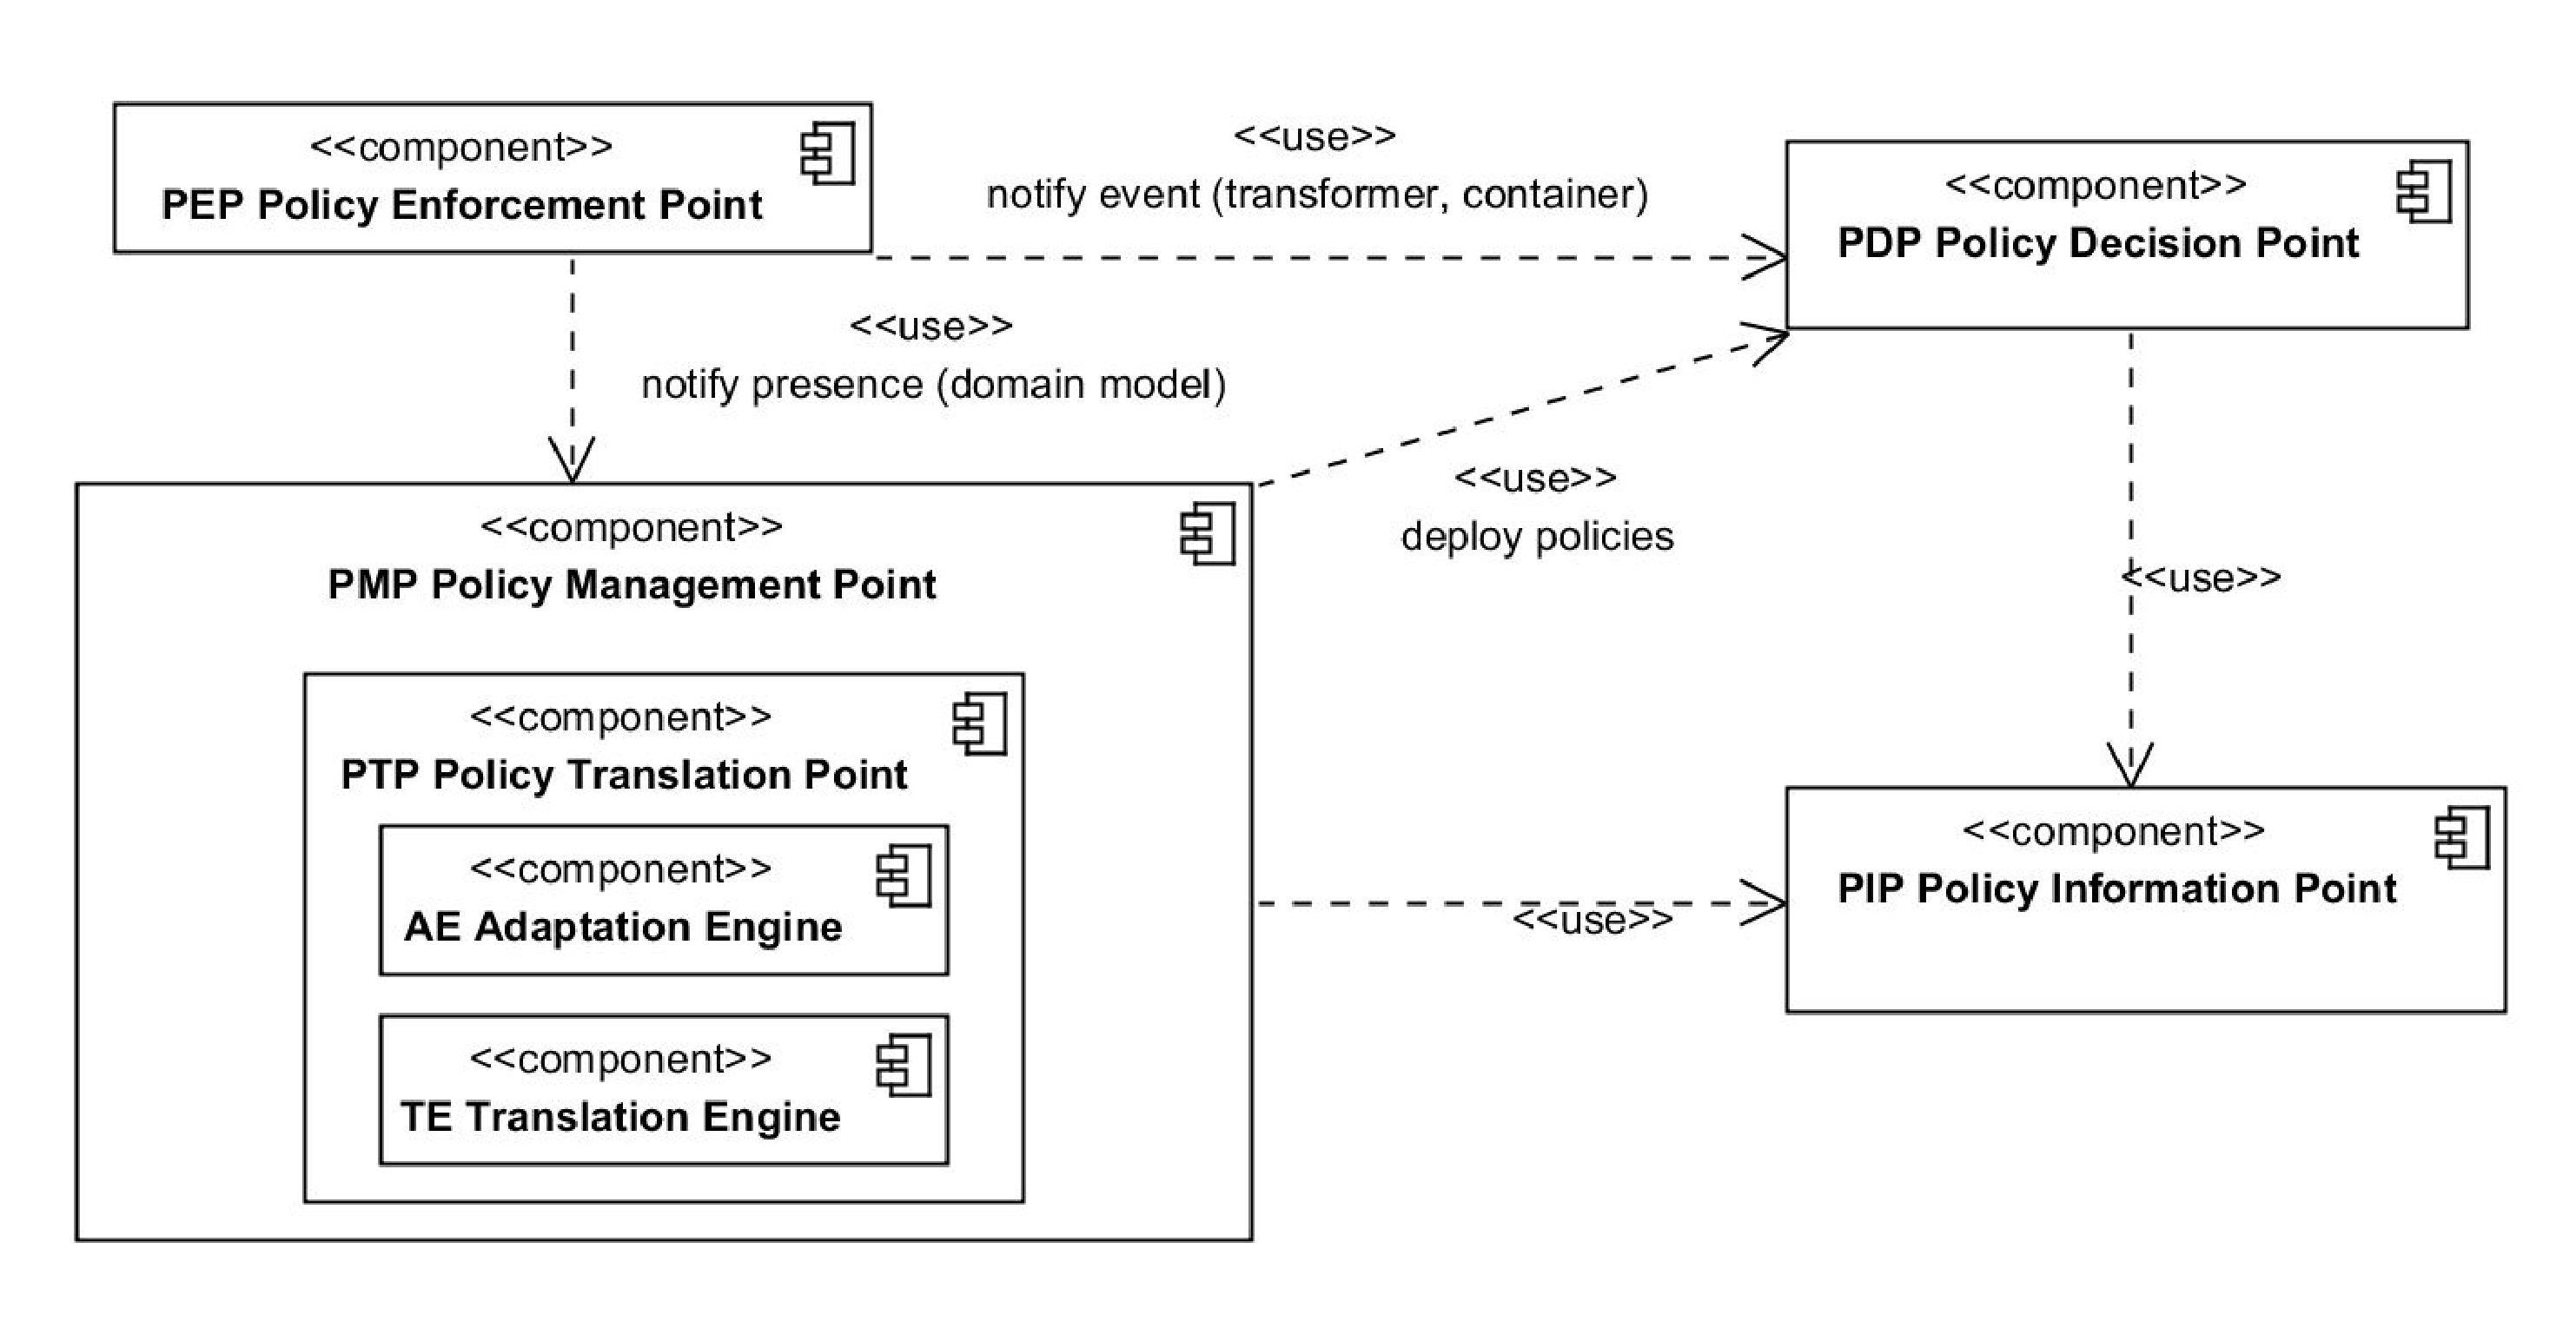
\epsfig{file=ptp.eps, height=1.7in, width=3in}
\caption{Usage Control infrastructure}
\label{fig:infrastructure}
\end{figure}

%----------------------------
\subsection{Initial conditions}
In an adaptive system environment one of the initial challenges is how to recognize change in the environment,
in our case how to recognize that the domain model has changed.
The first approach to recognize it, is in an active manner, labelled \textit{active notification},
meaning that the Usage Control (UC) infrastructure detects a new component and adds its domain-model to the UC infrastructure.
We recognized that this approach is not feasible because, for example,
on a machine there are some components which are installed and are not subject to the UC surveillance, such as Windows updates.
Other components that might be malware in nature are not detected upon installation. 
Also the UC infrastructure would have to broadcast a message and than listen for replies from newly added components.
This can impose performance penalties. 
Therefore, we opted for the next type of notification.
The second approach, labelled \textit{passive notification}, assumes that each component comes with its model
and it informs the system about its presence by sending its domain model as a parameter of the notification. 
Upon notification, the UC infrastructure incorporates the new elements which the new domain-model might have.

When a new PEP is added which requires a domain model correspondent,
the PEP will notify the PMP of its presence and will send the domain model and the refinement of its actions and transformers.
The new domain model always contains a three-layer model.
The core task of the Adaptation Engine, part of the PTP, is to recognize the differences and include them in the base domain model.

One has to consider also the cases when a domain model already contains the elements presented in the new domain model.
One approach is to override the existing elements with the new elements.
We have already seen that this approach can lead to a loss of information during refinement.
The second approach is to always include all the differences.
This has the disadvantage that the base domain model will increase in size rapidly and will end up containing deprecated elements.
But this approach has the advantage of backward compatibility. 
If policies are translated based on this model and later enforced on an older implementation, than they will still be correctly enforced.

The next step is to clearly define the initial conditions. 
The Usage Control infrastructure can start in one of two cases regarding the PTP. 
First, there is no initial model. In this case, the first installed PEP that notifies its presence will also deliver its domain model 
and this domain model will become the Base Domain Model for the entire infrastructure.
All additional PEPs when they will notify their presence to the infrastructure will have their domain model merged with the Base Model.
Secondly, the UC infrastructure has an initial model.
In this case, an administrator would have already defined an initial model for the infrastructure. 
All additional PEPs' Domain Models will be merged with the Base Model. 
This is the most common use case.

%----------------------------
\subsection{Adaptive behavior}
We have already mentioned that in order to provide automatic adaptation not only the domain model needs to be updated but also the policies.
This can be done with two approaches, we named them \textit{delayed} and \textit{real-time} adaptation.

The first approach is \textit{delayed adaptation}. This means that only when the Usage Control (UC) infrastructure is restarted and new policies are translated, 
will the new behavior be enforced. Until a system restart, the old policies are maintained. 
When a UC restart occurs and if the old policies have to be retranslated then the new model will be enforced. 

The second approach is \textit{real-time adaptation}. This means that after the domain model is merged, the old policies are retranslated and deployed,
and new policies will be translated according to the new domain model.
To achieve this we have also extended the behavior of the PMP.
Now, the PMP maintains a list with all the deployed policies and all the information necessary to automatically request a new translation from the PTP of a particular policy.
All the policies in the list are first revoked, then they are translated according to the new model and deployed to the PDP.

%===========================================
% SUBSECTION
%----------------------------
\subsection{Data and Containers}
While presenting the merging, we purposely left the PIM level the last, 
because here the data reflects entities from the user's business environment, the data one wants to protect
e.g. profile, blog, comment, budget, salary, income, expenses, insurance number.
In this case a simple string matching is not sufficient, because one domain can have a data named ``picture'' and another one ``photo''.
The adaptation engine has to recognize these two data as one and the same.
For this reason, we have used a natural language lexical library, namely Wordnet \cite{wordnet1, wordnet2, wordnet3} to establish relations between terms.
With this approach one can immediately establish relations between two terms.
Wordnet can also be used to identify relations of type \textit{part-of}, as in the case of album and photo.

The second challenge arose with those terms that talk of the same data with unrelated terms.
For example, if one social network has the concept ``wall'' while another one has the concept of ``mirror'' and these two networks merge,
than there is no direct linguistic relation between these terms. The updated domain model will use both of the terms.
In the case of similar data, we introduced the concept of an ``alias'' to a data, 
meaning that a data can have also a secondary name or even more which is a synonym to the primary name. 
The match between containers is done by comparing the name or the aliases of the data.
By using this mechanism and because the translation engine does a static translation based on the domain model,
the power-user can easily make connections between containers that at first did not have similar terms.
The policy being enforced in terms of implementation level is ignorant of the name of the data, because data was refined as a specific container, e.g file.

To compute the similarity between two words, the used library offers a multitude of algorithms to choose from to obtain a numerical value between two concepts.
We used the standard metric which takes into consideration the common parent and similar meaning to compute the value.
Taking into consideration the way the method to compute the distance and by using experimental methods we have also used a distance threshold from which the concepts can no longer be considered similar.

%===========================================
% SUBSECTION
%----------------------------
\subsection{Systems}

At the instance level, there is case when the domain model is not changed but a new instance of the same system is deployed.
For example, a new backup server is added to the network. The backup server has the same implementation details as the main server.
The PEP of this instance will notify its presence but the domain model has no new elements to be included.
The difference is where the protected data is stored.
In order that the UC control works correctly, the backup server must be populated with data via a monitored channel.
This means that the protected data is tracked by the UC infrastructure and the containers used on the new server to store the data are also traced by the UC infrastructure.
This monitoring has to be done at the Policy Information Point (PIP). 
If the system has a global PIP than it can maintain a map of all the allowed backups and all the containers where data may reside.
If the PIP is not global but local, than the policies which talk in terms of ``do action max/min/… number of times'' will not be enforced correctly if one access once the main back-up server, than the second back-up server and so on. This is avoided by using a centralized PIP. 
The state of the data is passed from one instance to another so that the PDP can correctly verify if the conditions specified in the policies are fulfilled.
The PDP has also to be centralized.

%===========================================
% SUBSECTION
%----------------------------
\subsection{Actions and Transformers}


%===========================================
% STUDY
\section{Case Study}
... not finished ...

Open systems, open-closed sys, closed sys
Closed – companies, controlled env. 
Open – facebook

Merge third-party with pim
Facebook : wall – guest book
Establish equivalence classes

User-specific ontology

%===========================================
% EVALUATION
\section{Evaluation}
%----------------------------
\subsection{Assumptions}

\begin{theorem}
Merging is done only at the same layer of abstraction. Only elements pertaining to the same system are merged
\label{assumption1}
\end{theorem}

\begin{theorem}
Always the maximum security level is enforced.
\label{assumption2}
\end{theorem}

\begin{theorem}
At PSM and ISM for the same system, the terminology follows a common vocabulary.
\label{assumption3}
\end{theorem}

%----------------------------
\subsection{Limitations}
The data from a domain model could be specified with business domain terms which are not recognized by a lexical ontology.
Therefore, a specific use case ontology should be put in place.

The domain model is always updated and backward compatibility is maintained.
This means that the base domain model always expands.
In case a domain model must be simplified, this must be done either manually or
by using a special notification signed by the administrator to mark that the new domain model must be accepted as a replacement
for the elements it contains.

%----------------------------
\subsection{Performance}
The only technical evaluation that comes to my mind is “performance”.
Apart from this, you must write down the assumptions and the limitations as part of security and correctness analysis.
As for evaluation of your work, we will do performance analysis. Please think what you would like to test there. 
It’s very important in any type of evaluation to evaluate the correct parameters.
We will need some discussion and argument there as to why we chose to measure one thing and not the other (if that is the case).
%===========================================
% RELATED
\section{Related work}

... not finished ...

I don't think it's useful at this moment to spend time reading this section ...

Paper 2. Ontology-based Policy Refinement Using SWRL Rules for Management Information Definitions in OWL
The present work presents an approach on how ontology representation could be used for dynamic policy interoperability between HL business rules and LL network policies, while maintaining the separation of concepts of HL and LL information. 
This approach does not attempt to directly translate policies from the upper level into a set of policies or configuration commands at the lower level.
* describes PIM to ISM mapping by using ontologies

Paper 3. Information Domain Modeling for Adaptive Web Systems
This paper presents a Domain Modeling System, which builds a domain model framework for adaptive Web systems. It records concepts and the relationships among them and represents them as a concept network. To speed up run time searches, the system finds all related concepts by calculating the optimal paths between all pairs of concepts offline in advance. 
Domain independent relationships
The types of relations could be established between the elements in the domains we want to merge. Further study and thinking on this required.
Discovered Relationships
1. Association(a,b): 

Paper 4. Ontology Merging for Federated Ontologies on the Semantic Web – 2001
We propose the new method FCA–MERGE for merging ontologies following a bottom-up approach which offers a global structural description of the merging process. There is no common formal definition of what an ontology is. However, most approaches share a few core items: concepts, a hierarchical IS-A-relation, and further relations.
This architecture is similar with what we want to have. An ontology is a Domain Model. New components are added to the system with their own DM, which in this figure is portrayed by the local ontology. The merged ontology is the merged Domain Model which will be stored on the Translation Engine.
Bottom-Up Ontology Merging
Our mechanism is based on application-specific instances of the two given ontologies O1 and O2 that are to be merged. 

Paper 6. XML Schema Element Similarity Measures: A Schema Matching Context
2009 - Alsayed Algergawy, RichiNayak, and Gunter Saake
In this paper, we classify, review, and experimentally compare major methods that are exploited in the definition, adoption, and utilization of element similarity measures in the context of XML schema matching. 
This work focuses on measuring the similarity between whole XML data not on the individual elements. In this paper, we aim to classify, review, and experimentally compare element similarity measures in the context of XML schema matching.
Element names can be syntactically similar (Staff, TechnicalStaff) or semantically similar (People, Staff). To determine the similarity between a pair of tokens, sim(t1,t2), both syntactic and semantic measures can be used.

Paper 7. String similarity Metrics for Ontology Alignment
2013
Probabilistic approaches
In our system, we cannot use probabilistic approaches in establishing relation between elements. The relation must be well defined. If we use probabilistic approaches and two nodes are similar in terms of semantics, in reality this might introduce security vulnerabilities. For example, if delete is refined as delete data and overwrite after 3 times, and another delete is refined only overwrite once, than it might be possible for the second case to recover the data. The refinement of the copy is similar between the two versions of the copy. A probabilistic approach will recognize these two refinements as similar and use just one of them. 


- no model based-policy translation ?

- no runtime adaptve usage control infrastructures ?

- no business specific ontologies ?


%===========================================
% CONCLUSIONS
\section{Conclusions and Future Work}
... not finished ...

This paragraph will end the body of this sample document.
Remember that you might still have Acknowledgments or
Appendices; brief samples of these
follow.


%\end{document}  % This is where a 'short' article might terminate


%
% The following two commands are all you need in the
% initial runs of your .tex file to
% produce the bibliography for the citations in your paper.
%===========================================
%BIBLIOGRAPHY
\bibliographystyle{abbrv}

\begin{thebibliography}{4}

\bibitem{workshop1} A. Pretschner, E. Lovat, M. Buechler: Representation-Independent Data Usage Control, in
\textit{Sixth International Workshopon Data Privacy Management}, pp.29, 2011

\bibitem{proceeding2} M. Hilty, D. Basin, C. Schaefer, T. Walter, J. Biskup, and J. L\`{o}pez : A Policy Language for Distributed Usage Control, in
\textit{Proc. 12th European  Symp. on Research in Computer Security}, vol. 4734, pp.531-546, 2007

\bibitem{conference3} Pretschner, A.: An Overview of Distributed Usage Control, in
\textit{Knowledge Engineering: Principles and Techniques Conference}, pp.25-33, 2009

\bibitem{proceeding4} P. Kumari, A. Pretschner: Model-based Usage Control Policy Derivation, 
\textit{Proc. 5th International Symposium on Engineering Secure Software and Systems (ESSoS)}, pp.58-74, February, 2013

\bibitem{proceeding5} P. Kumari, A. Pretschner: Deriving Implementation-level Policies for Usage Control Enforcement, 
\textit{Proc. 2nd ACM Conference on Data and Application Security and Privacy (CODASPY)}, pp.83-94, February, 2012

\bibitem{icse9} Ji Zhang, Betty H. C. Cheng: Model-based development of dynamically adaptive software, 
\textit{ICSE}, pp.371-380, 2006

\bibitem{proceeding10} Betty H. C. Cheng, P. Sawyer, N. Bencomo, J. Whittle: A Goal-Based Modeling Approach to Develop Requirements of an Adaptive System with Environmental Uncertainty, 
\textit{Proceedings of the ACM/IEEE International Conference on Model Driven Engineering Languages and Systems (MoDELS 2009)}, pp.468-483, 2009

\bibitem{adaptive1} Betty H. Cheng, R. Lemos, H. Giese et al.: Software Engineering for Self-Adaptive Systems: A Research Roadmap, 
\textit{Software Engineering for Self-Adaptive Systems, Springer}, pp.1-26, 2009

\bibitem{adaptive2} R. Lemos, H. Giese, M. Shaw et al.: Software Engineering for Self-Adaptive Systems: A Second Research Roadmap, 
\textit{Software Engineering for Self-Adaptive Systems : Lecture Notes in Computer Science Volume 7475, Springer}, pp.1-32, 2013

\bibitem{wordnet1} George A. Miller: WordNet: A Lexical Database for English, 
\textit{Communications of the ACM Vol. 38}, No. 11, pp.39-41, 1995

\bibitem{wordnet2} Christiane Fellbaum: WordNet: An Electronic Lexical Database, 
\textit{Cambridge, MA: MIT Press.}, 1998

\bibitem{wordnet3} RiTa.WordNet: Java library to access to the WordNet ontology, 
\textit{http://rednoise.org/rita/index.html}

\bibitem{book1} Ontology Matching, 
\textit{Springer, 2nd. ed}, 2013

\bibitem{proceeding11} Wenpu Xing; Ghorbani, A.A.: Information domain modeling for adaptive Web systems,
\textit{Proc. IEEE/WIC/ACM International Conference on Web Intelligence}, pp.684-687, 2005

\bibitem{Uml1} Szlenk, M.: Formal Semantics and Reasoning about UML Class Diagram,
\textit{Proc. IEEE Dependability of Computer Systems}, pp.51-59, 2006


\end{thebibliography}  

%\balancecolumns

\balancecolumns
% That's all folks!
\end{document}
